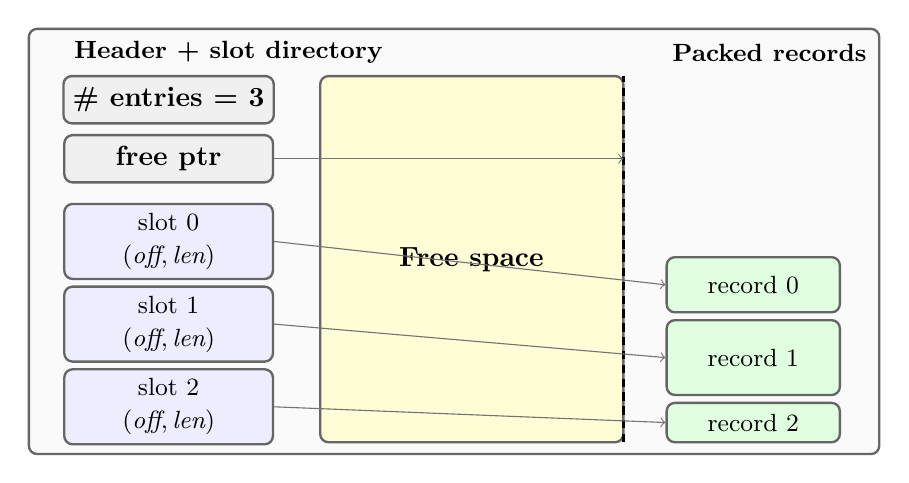
\begin{tikzpicture}[
    x=1cm,y=1cm,
    every node/.style={font=\small},
    frame/.style={draw=black!60, rounded corners=3pt, line width=0.85pt},
    header/.style={frame, fill=gray!12, minimum width=2.65cm, minimum height=0.6cm, align=center, font=\bfseries},
    slot/.style={frame, fill=blue!7, minimum width=2.65cm, minimum height=0.9cm, align=center},
    free/.style={frame, fill=yellow!16},
    rec/.style={frame, fill=green!12, minimum width=2.2cm, align=center},
    link/.style={->, thin, draw=black!55}
]
    \draw[frame, fill=gray!4] (0,0) rectangle (10.8,5.4);

    \node[anchor=west, font=\bfseries\small] at (0.45,5.10) {Header + slot directory};
    \node[anchor=west, font=\bfseries\small] at (8.05,5.10) {Packed records};

    \node[header] (h1) at (1.775,4.50) {\# entries = 3};
    \node[header] (h2) at (1.775,3.75) {free ptr};

    \node[slot] (s0) at (1.775,2.70) {slot 0\\[0.1em]$(\textit{off},\textit{len})$};
    \node[slot] (s1) at (1.775,1.65) {slot 1\\[0.1em]$(\textit{off},\textit{len})$};
    \node[slot] (s2) at (1.775,0.60) {slot 2\\[0.1em]$(\textit{off},\textit{len})$};

    \draw[free] (3.70,0.15) rectangle (7.55,4.80);
    \node[font=\bfseries] at (5.62,2.47) {Free space};
    \draw[densely dashed, line width=0.9pt] (7.55,0.15) -- (7.55,4.80);
    \draw[link] (h2.east) -- (7.55,3.75);

    \node[rec, minimum height=0.7cm] (r0) at (9.20,2.15) {record 0};
    \node[rec, minimum height=0.95cm] (r1) at (9.20,1.225) {record 1};
    \node[rec, minimum height=0.5cm] (r2) at (9.20,0.40) {record 2};

    \draw[link] (s0.east) -- (r0.west);
    \draw[link] (s1.east) -- (r1.west);
    \draw[link] (s2.east) -- (r2.west);
\end{tikzpicture}
